\documentclass[letterpaper]{article}
\usepackage{calc,amsmath,amssymb,amsfonts}
\usepackage{graphicx}
\usepackage[T1]{fontenc}
\usepackage[french,spanish]{babel}
\usepackage[x11names]{xcolor}

\usepackage[fancyhdr]{geometry}
\usepackage{enumitem,hyperref}
\usepackage{float}
\hypersetup{colorlinks=true,allcolors=blue,pdftitle=1,pdfauthor=Mauricio Guerrero}
\documentclass[letterpaper]{article}
\usepackage{calc,amsmath,amssymb,amsfonts}
 \usepackage{graphicx} 
\usepackage[T1]{fontenc}
\usepackage{pgfgantt}
\usepackage{booktabs}
\usepackage{tabularx}
\renewcommand{\arraystretch}{1.1} % Aumenta el alto de las filas

\usepackage[margin=1in]{geometry}
\usepackage[french,spanish]{babel}
\usepackage{xcolor,fancyhdr}
\usepackage[vmargin=0.3937in,left=1.1811in,right=0.9846in,includeheadfoot,head=0.4925in,headsep=0.4528in,foot=0.4925in,footskip=0.9453in]{geometry}
\usepackage{enumitem,hyperref}
\hypersetup{colorlinks=true,allcolors=blue,pdftitle=1,pdfauthor=Mauricio Guerrero}
% Outline numbering
\setcounter{secnumdepth}{5}
\renewcommand\thesection{\arabic{section}}
\renewcommand\thesubsection{\arabic{section}.\arabic{subsection}}
\renewcommand\thesubsubsection{\arabic{section}.\arabic{subsection}.\arabic{subsubsection}}
\renewcommand\theparagraph{\arabic{section}.\arabic{subsection}.\arabic{subsubsection}.\arabic{paragraph}}
\renewcommand\thesubparagraph{\arabic{section}.\arabic{subsection}.\arabic{subsubsection}.\arabic{paragraph}.\arabic{subparagraph}}
% Pages
\fancypagestyle{Convertedi}{\fancyhf{}
  \fancyhead[R]{}
  \fancyfoot[L]{}
  \renewcommand\headrulewidth{0pt}
  \renewcommand\footrulewidth{0pt}
  \renewcommand\thepage{\arabic{page}}
}
\fancypagestyle{Standard}{\fancyhf{}
  \fancyhead[L]{\hfill \hfill \hfill \hfill \thepage{}}
  \fancyfoot[L]{}
  \renewcommand\headrulewidth{0pt}
  \renewcommand\footrulewidth{0pt}
  \renewcommand\thepage{\arabic{page}}
}
\fancypagestyle{FirstPage}{\fancyhf{}
  \fancyhead[L]{}
  \fancyfoot[L]{}
  \renewcommand\headrulewidth{0pt}
  \renewcommand\footrulewidth{0pt}
  \renewcommand\thepage{\arabic{page}}
}
\pagestyle{Standard}
\title{1}
\author{Mauricio Guerrero}
\date{2010-11-17}
\begin{document}
\clearpage
\pagestyle{Standard}
\thispagestyle{FirstPage}
\setcounter{page}{1}
{\selectlanguage{french}
\foreignlanguage{spanish}


\bigskip


\bigskip

{\centering\selectlanguage{french}
\foreignlanguage{spanish}{\textbf{PROPUESTA PROYECTO FIN DE CARRERA}}
\par}


\bigskip

{\centering\selectlanguage{french}
\foreignlanguage{spanish}{Presentado a}
\par}


\bigskip

{\centering\selectlanguage{french}
\foreignlanguage{spanish}{\textbf{LA UNIVERSIDAD DE LOS ANDES}}
\par}

{\centering\selectlanguage{french}
\foreignlanguage{spanish}{\textbf{FACULTAD DE INGENIERÍA}}
\par}

{\centering\selectlanguage{french}
\foreignlanguage{spanish}{\textbf{DEPARTAMENTO DE INGENIERÍA ELÉCTRICA Y ELECTRÓNICA}}
\par}


\bigskip


\bigskip


\bigskip

{\centering\selectlanguage{french}
\foreignlanguage{spanish}{Para obtener el título de}
\par}


\bigskip

{\centering\selectlanguage{french}
\foreignlanguage{spanish}{\textbf{INGENIERO ELECTRÓNICO}}
\par}


\bigskip


\bigskip

{\centering\selectlanguage{french}
\foreignlanguage{spanish}{por }
\par}


\bigskip

{\centering\selectlanguage{french}
\foreignlanguage{spanish}{\textbf{\textit{Sergio Andrés Arroyo Cruzco}}}
\par}


\bigskip


\bigskip


\bigskip


\bigskip

{\centering\selectlanguage{french}
\foreignlanguage{spanish}{\textbf{\textit{Propuesta de lazo de control de un convertidor DC DC bidireccional en configuración interleaved usando HIL}}}
\par}


\bigskip


\bigskip


\bigskip

{\centering\selectlanguage{french}
\foreignlanguage{spanish}
\par}


\bigskip


\bigskip




\bigskip


\bigskip

{\selectlanguage{spanish}
\foreignlanguage{spanish}{\textit{{}-\ \ \ \ Asesor}}\foreignlanguage{spanish}{:\ \ \ \ \ Guillermo Andres Jimenez Estevez, Profesor
Asociado, Universidad de Los Andes}}



\clearpage
\pagestyle{Convertedi}
{\selectlanguage{spanish}\bfseries\color[HTML]{365F91}
\foreignlanguage{spanish}{{Contenido}}

\setcounter{tocdepth}{3}
\tableofcontents}

\clearpage\section{Caracterización del problema (Justificación)}
El creciente interés en las energías renovables, el almacenamiento energético y la electrificación de sectores estratégicos ha impulsado la necesidad de desarrollar sistemas de conversión de potencia más eficientes, precisos y confiables. En este contexto, los convertidores DC-DC bidireccionales juegan un papel fundamental, ya que permiten gestionar el flujo de energía en ambos sentidos entre distintas fuentes y cargas de corriente continua. Estos convertidores son clave en aplicaciones como sistemas de baterías (BESS), vehículos eléctricos, sistemas fotovoltaicos y microrredes DC, donde la precisión y robustez en el control son requisitos esenciales.

Las microrredes DC presentan ventajas significativas en términos de eficiencia y compatibilidad con fuentes renovables, pero su correcto funcionamiento depende de la implementación de sistemas de control sofisticados para los convertidores asociados. Particularmente, la topología de puente medio bidireccional en configuración interleaved ha demostrado potencial para mejorar la calidad del rizado de corriente, la distribución térmica y la respuesta dinámica del sistema. Sin embargo, el diseño e implementación del lazo de control para esta configuración requiere una cuidadosa coordinación de fases y una validación rigurosa.

En este sentido, aunque existen estudios teóricos y simulaciones, la validación experimental mediante entornos Hardware-in-the-Loop (HIL) sigue siendo un área con amplio potencial de desarrollo. El uso de HIL permite realizar pruebas en tiempo real de los algoritmos de control, combinando simulaciones precisas con hardware físico, lo que facilita la identificación y corrección de fallas antes de la implementación final.

Por lo tanto, esta tesis se enfoca en la propuesta, diseño y validación de un lazo de control para un convertidor DC-DC bidireccional en configuración interleaved, utilizando una plataforma HIL. Esta aproximación permitirá evaluar integralmente el desempeño del sistema bajo condiciones realistas, contribuyendo al avance en el control electrónico de convertidores y fortaleciendo su aplicabilidad en microrredes DC y otros sistemas donde la conversión bidireccional es crítica.
\section{Marco Teórico}

\subsection{Antecedentes externos}

La configuración interleaved en convertidores DC-DC bidireccionales se ha consolidado como una técnica efectiva para mejorar el rendimiento energético y reducir las pérdidas por conmutación. Al operar varias fases desfasadas, esta topología permite reducir la frecuencia de conmutación percibida en cada inductor, lo que disminuye el estrés térmico y eléctrico sobre los componentes. Investigadores en China, como se presenta en \cite{liu2023interleaved}, demostraron que un convertidor buck interleaved de tres fases con inductores acoplados operando a 500 kHz puede alcanzar una eficiencia superior al 98\%, gracias a la reducción del rizado de corriente y la mejora en la distribución de las cargas entre fases. De manera similar, en India, Banerjee et al.~\cite{banerjee2024sic} estudiaron un convertidor buck interleaved de dos fases que utiliza MOSFETs de carburo de silicio (SiC) junto con inductores acoplados, evidenciando una notable reducción en el rizado de corriente y una mejor respuesta dinámica del sistema.\\
El impacto de la configuración interleaved también se observa en la reducción del valor de inductancia requerida y en la mejora del control del rizado de corriente. Nuevamente en China, Liu et al.~\cite{liu2023interleaved} desarrollaron un modelo que relaciona el coeficiente de acoplamiento en inductores integrados con la inductancia equivalente, mostrando cómo un mayor acoplamiento magnético contribuye a minimizar el rizado y a mejorar la eficiencia global del convertidor. De manera similar, en Estados Unidos, en ~\cite{duan2023multiphase} analizaron un convertidor DC-DC bidireccional interleaved con fases variables, donde el ajuste del número de fases y el ciclo de trabajo permite optimizar el rizado de corriente, mejorando la calidad del flujo energético y disminuyendo pérdidas. Estos estudios internacionales respaldan la aplicación de configuraciones interleaved para lograr convertidores más eficientes, compactos y con mejor rendimiento térmico y eléctrico.


\subsection{Antecedentes locales}

En Colombia, se han realizado aportes significativos en el control de convertidores DC-DC bidireccionales. Por ejemplo, en \cite{narvaez2024hess} se presenta un tesis, la cual se destaca por su enfoque en el diseño y validación de algoritmos de control digital adaptativo para convertidores bidireccionales de puente medio, enfatizando la robustez ante variaciones en las condiciones de carga y las perturbaciones externas. Su trabajo incluye la implementación de lazos de control basados en técnicas avanzadas de control predictivo y adaptativo, orientados a optimizar la respuesta dinámica y la estabilidad del sistema bajo escenarios reales de operación.\\
Por otro lado, en \cite{yate2024control} se profundiza en el desarrollo de estrategias de control digital para convertidores DC-DC bidireccionales en configuración interleaved, utilizando plataformas Hardware-in-the-Loop (HIL) para validar el desempeño de los controladores propuestos. Esta investigación pone especial énfasis en la coordinación de fases y la minimización del rizado de corriente mediante la modulación del ciclo de trabajo y el control en tiempo real, aspectos fundamentales para extender la vida útil de los dispositivos de potencia y mejorar la eficiencia energética en sistemas de almacenamiento de energía.\\
Finalmente, una contribución adicional proviene de \cite{gomez2023control} de la Universidad Nacional de Colombia, quienes desarrollaron un modelo de control híbrido para convertidores bidireccionales que combina control clásico y técnicas de inteligencia artificial para la optimización adaptativa del ciclo de trabajo en convertidores interleaved. Su estudio incluye análisis de estabilidad y validación experimental en prototipos físicos, lo que aporta un marco práctico para la aplicación de control avanzado en entornos reales de microrredes DC.

\section{Caracterización del proyecto}

\subsection{Objetivo general}
Diseñar, implementar y validar un lazo de control para un convertidor DC-DC bidireccional en configuración interleaved, optimizando la reducción de la inductancia y el rizado de corriente, utilizando una plataforma HIL para su validación en tiempo real.
\subsection{Objetivos específicos}
\begin{itemize}
    \item Justificar y demostrar que la configuración interleaved permite reducir a la mitad la frecuencia efectiva de operación del convertidor.

    \item Analizar cómo la reducción en la frecuencia de conmutación impacta en el valor requerido de la inductancia, permitiendo utilizar inductores de menor tamaño y costo sin comprometer el rendimiento.

    \item Evaluar la disminución del rizado de corriente mediante la combinación de corrientes desfasadas de las fases interleaved, mejorando la calidad de la señal y reduciendo las pérdidas térmicas.

    \item Desarrollar e implementar el lazo de control que sincronice y coordine ambas fases para maximizar los beneficios de la configuración interleaved en términos de reducción de rizado y eficiencia.
\end{itemize}







\subsection{Alcance}

\section{Contexto del proyecto y tratamientos}

\subsection{Suposiciones}

\begin{itemize}
  \item Se asume que los modelos matemáticos y de control desarrollados representan con suficiente precisión el comportamiento dinámico del convertidor y sus componentes.
  \item Se supone que la plataforma HIL es compatible y permitirá una integración efectiva con el hardware físico del convertidor.
  \item Se considera que los módulos físicos del convertidor están disponibles y cumplen con las especificaciones técnicas necesarias para la implementación y pruebas.
  \item Se asume que las condiciones de operación simuladas y experimentales serán representativas de escenarios reales de funcionamiento en microrredes y sistemas de almacenamiento de energía.
    \item Se considera que la resolución temporal y capacidad de procesamiento de la plataforma HIL son suficientes para replicar con precisión el comportamiento dinámico del sistema real.

\end{itemize}

\subsection{Restricciones}

\begin{itemize}
  \item El desarrollo experimental del proyecto depende de la disponibilidad de los módulos físicos de H-Bridge.
  \item El acceso al laboratorio, equipos y soporte técnico de la universidad Distrital está condicionado a los tiempos, políticas y disponibilidad de los profesores y personal de apoyo.
  \item El cronograma del proyecto puede verse afectado por los trámites administrativos requeridos para el ingreso y utilización de los recursos en la universidad colaboradora.
  \item Las pruebas físicas del convertidor en configuración interleaved estarán limitadas al equipamiento previamente disponible, sin posibilidad de rediseño estructural de hardware.


\end{itemize}

\subsection{Factores de riesgo}

\begin{itemize}
  \item Posibles demoras en la disponibilidad de los módulos o recursos necesarios en la universidad colaboradora, lo cual podría retrasar la etapa de implementación y validación.
  \item Restricciones administrativas o logísticas que dificulten el acceso oportuno a laboratorios o equipamiento.
  \item Incompatibilidad entre la plataforma HIL del proyecto y el diseño físico de los módulos existentes, lo cual podría requerir adaptaciones técnicas imprevistas.
  \item Riesgos asociados al transporte, manipulación o fallas en los módulos físicos que comprometan el desarrollo del prototipo interleaved.
\end{itemize}



\section{Cronograma}

\begin{figure}[H]
    \centering
    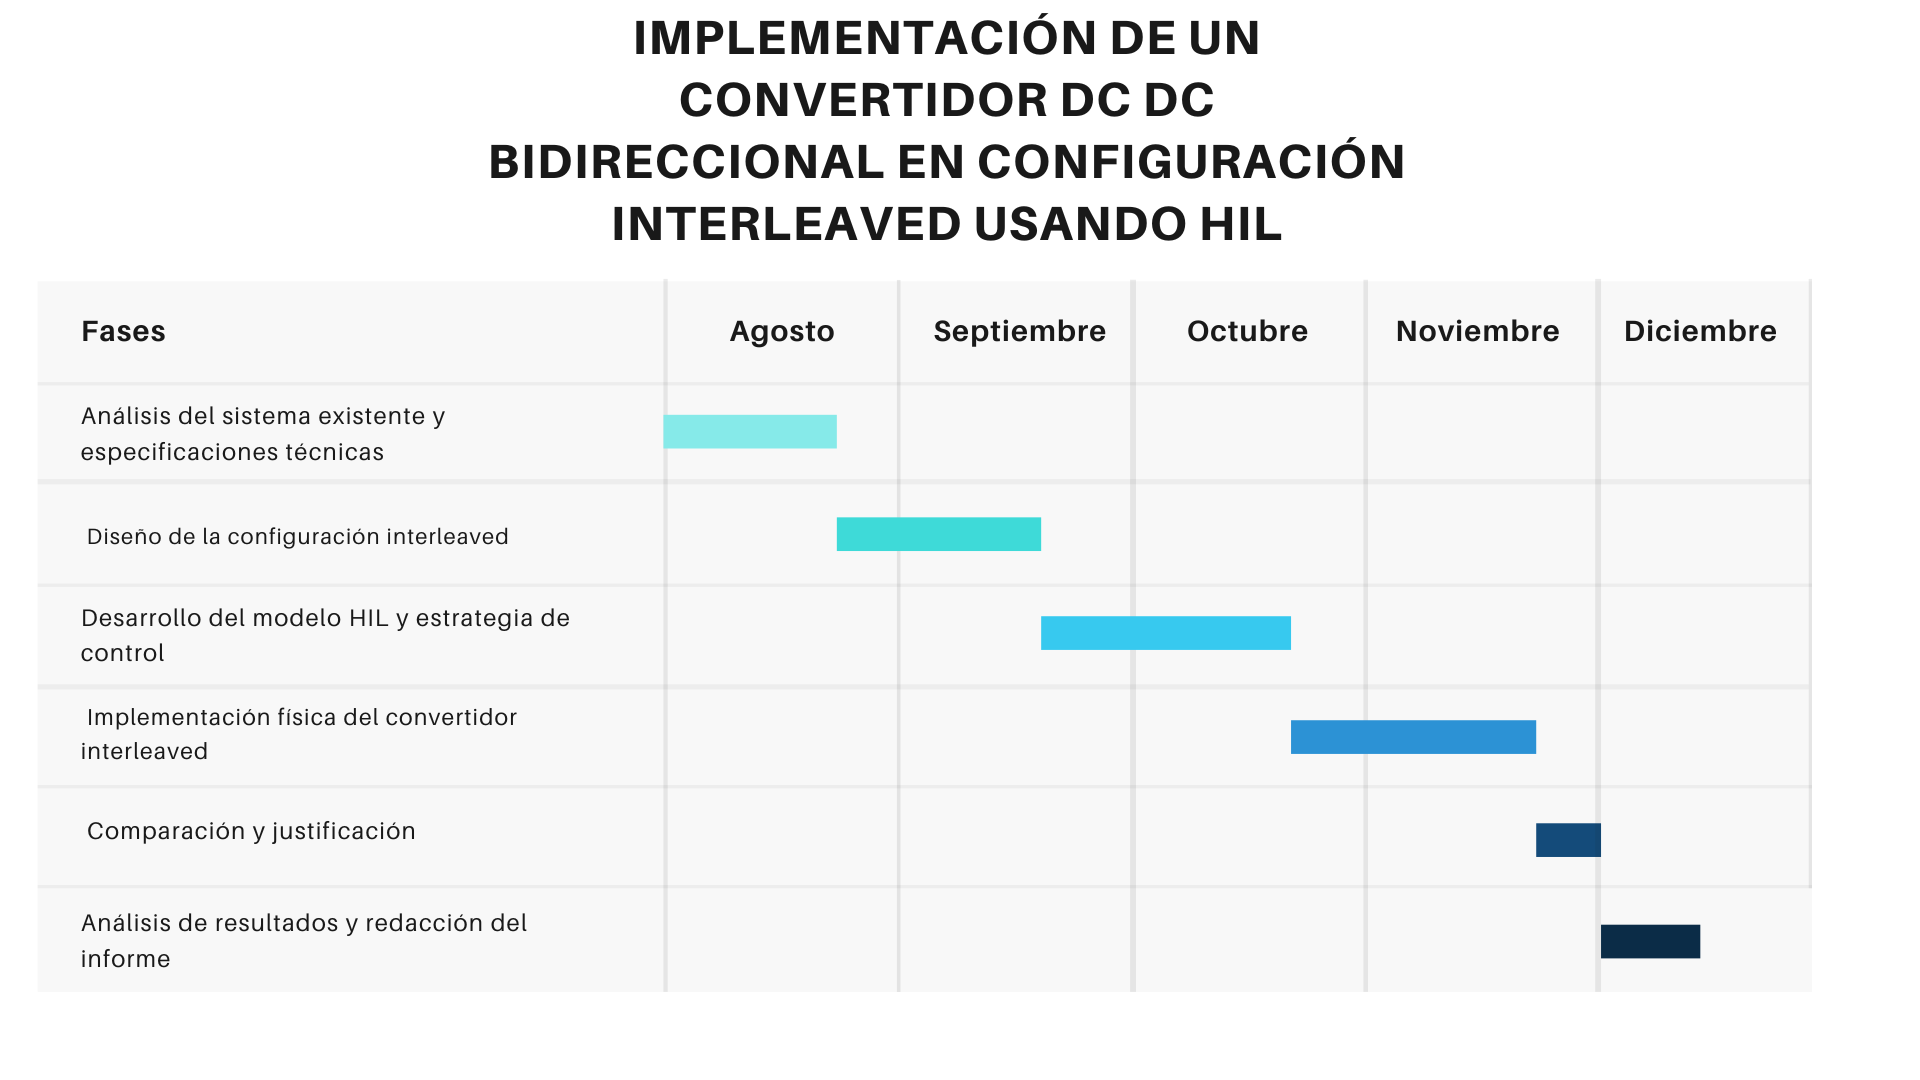
\includegraphics[width=0.9\linewidth]{imgs/Gantt Chart.png}
    \caption{Fases a realizar para el proyecto de grado}
    \label{fig:enter-label}
\end{figure}

\subsection{Identificación y descripción de hitos}


A continuación se describen los hitos clave del proyecto
\renewcommand{\tablename}{Tabla}
\begin{table}[H]
\small % Reduce el tamaño de la letra dentro de la tabla
\begin{tabularx}{\textwidth}{|c| l| X| l|}
\specialrule{1pt}{1pt}{1pt}
\textbf{Nº} & \textbf{Fase} & \textbf{Hito} & \textbf{Fecha estimada} \\
\specialrule{1pt}{1pt}{1pt}
1 & Fase 1 & Inicio del proyecto y levantamiento de información técnica de los módulos físicos existentes. & 4 de agosto de 2025 \\ \hline
2 & Fase 1 & Identificación de parámetros eléctricos (tensión, corriente, frecuencia). & 11 de agosto de 2025 \\ \hline
3 & Fase 2 & Selección de módulos y diseño preliminar de conexión interleaved. & 25 de agosto de 2025 \\ \hline
4 & Fase 2 & Simulación inicial del convertidor interleaved. & 10 de septiembre de 2025 \\ \hline
5 & Fase 3 & Modelado del convertidor interleaved en entorno HIL. & 20 de septiembre de 2025 \\ \hline
6 & Fase 3 & Implementación de control digital y validación HIL. & 10 de octubre de 2025 \\ \hline
7 & Fase 4 & Montaje físico e integración de los módulos en configuración interleaved. & 20 de octubre de 2025 \\ \hline
8 & Fase 4 & Pruebas con cargas reales (baterías y supercondensadores). & 5 de noviembre de 2025 \\ \hline
9 & Fase 5 & Evaluación técnica y comparación con el puente medio tradicional. & 20 de noviembre de 2025 \\ \hline
10 & Fase 6 & Entrega del documento final de tesis. & 10 de diciembre de 2025 \\
\specialrule{1pt}{1pt}{1pt}
\end{tabularx}
\end{table}

\section{Recursos}

Para el desarrollo del presente proyecto de tesis, se contará con una combinación de herramientas de software, plataformas de simulación en tiempo real y equipos físicos. A continuación, se describen los recursos principales requeridos y su función específica dentro del proyecto:

\begin{itemize}
    \item \textbf{MATLAB/Simulink:} Se utilizará para la simulación inicial del convertidor bidireccional en configuración interleaved. Permitirá validar el comportamiento teórico del sistema, afinar parámetros de diseño y modelar las estrategias de control antes de su implementación en la plataforma HIL.

    \item \textbf{Plataforma OPAL-RT:} Se empleará como entorno de simulación en tiempo real para validar el comportamiento del convertidor bajo condiciones similares a las reales, permitiendo probar la respuesta del sistema frente a distintos escenarios sin riesgo para los equipos físicos.

    \item \textbf{Microsoft Excel:} Herramienta de apoyo para la organización de datos experimentales, análisis estadístico básico, procesamiento de resultados de simulaciones y generación de tablas y gráficas para la documentación del proyecto.

    \item \textbf{Módulos físicos de puente medio:} Proporcionados por la universidad colaboradora. Se utilizarán dos módulos para su conexión en paralelo bajo configuración interleaved, permitiendo implementar la topología estudiada de forma física y evaluar su comportamiento real.

    \item \textbf{Sistema de almacenamiento de energía (baterías y supercondensador):} Forman parte de la microrred DC existente y permitirán realizar pruebas prácticas de carga y descarga utilizando el convertidor implementado.

    \item \textbf{Fuente bidireccional DC/DC:} Fuente programable que permitirá inyectar o absorber potencia desde el sistema, simulando diferentes condiciones de operación y facilitando pruebas controladas del convertidor.

    \item \textbf{Instrumentación de laboratorio (osciloscopios, multímetros, fuente de alimentación, cargas electrónicas, etc.):} Utilizada para la medición de variables eléctricas clave (tensión, corriente, rizado), validación de señales de control y verificación del funcionamiento físico del convertidor implementado.
\end{itemize}








\section*{Anexos}


\begin{itemize}
    \item Presentación de propuesta de grado firmada por el asesor académico, profesor Guillermo Jiménez.
    \item Autorización de uso del trabajo a favor de la Universidad de los Andes.
\end{itemize}


\renewcommand{\refname}{Referencias}
\bibliographystyle{IEEEtran}
\bibliography{bibliografia} % Reemplaza tureferencias por el nombre real de tu archivo .bib

\end{document}


